\documentclass[spanish,a4paper,12pt,twoside,openright]{extreport}

\usepackage[dvips]{graphicx}
\usepackage[dvips]{epsfig}
\usepackage[utf8]{inputenc}
\usepackage[spanish]{babel}
\usepackage{alltt}

\usepackage[ruled,vlined,commentsnumbered,linesnumbered,inoutnumbered,titlenotnumbered,noend]{algorithm2e}
\SetKwRepeat{Do}{do}{while}

\usepackage{multirow}
\usepackage{adjustbox}
\usepackage{array} 
\usepackage{amsfonts}
\usepackage{amsmath}
\usepackage{bigstrut}
\usepackage{booktabs}
\usepackage{caption}
\usepackage{chngpage}
\usepackage{float}
\usepackage{lipsum}
\usepackage{graphicx}
\usepackage{lscape}
\usepackage{microtype}
\usepackage[numbers]{natbib}
\usepackage{pdflscape}
\usepackage{rotating}
\usepackage{subcaption}
\usepackage{ctable}
\usepackage{enumerate}
\usepackage{gensymb}
\usepackage{eurosym}
\usepackage{xcolor}
\usepackage{tabu}
\usepackage{lineno}
\usepackage{hyperref}
\usepackage[top=2cm, bottom=2cm, left=2cm, right=2cm]{geometry}

\newenvironment{sourcecode}
{\begin{list}{}{\setlength{\leftmargin}{1em}}\item\scriptsize\bfseries}
{\end{list}}

\newenvironment{littlesourcecode}
{\begin{list}{}{\setlength{\leftmargin}{1em}}\item\tiny\bfseries}
{\end{list}}

\newenvironment{abstract_en}
{\par\noindent\begin{center}\textbf{Abstract}\end{center}\begin{itshape}\par\noindent}
{\end{itshape}}

\newenvironment{keywords}
{\begin{list}{}{\setlength{\leftmargin}{1em}}\item[\hskip\labelsep \bfseries Keywords:]}
{\end{list}}

\newenvironment{palabrasClave}
{\begin{list}{}{\setlength{\leftmargin}{1em}}\item[\hskip\labelsep \bfseries Palabras clave:]}
{\end{list}}

\usepackage{bera}% optional: just to have a nice mono-spaced font
\usepackage{listings}
\usepackage{xcolor}

\colorlet{punct}{red!60!black}
\definecolor{background}{HTML}{EEEEEE}
\definecolor{delim}{RGB}{20,105,176}
\colorlet{numb}{magenta!60!black}

\lstdefinelanguage{Csharp}{
  morekeywords = {public, private, class, using, void, var, this, get, set, new, if, else, foreach, in, bool, int, string, float, double, static, return, true, false},
  morecomment = [l]{//},
  morecomment = [s]{/}{/},
  morestring = [b]",
  sensitive = true
}

\lstdefinestyle{basicStyle}{
  basicstyle=\ttfamily\color{black},
  commentstyle=\color{black},
  tabsize=2
}

\lstset{
  language=[Sharp]C,
  basicstyle=\ttfamily\small,
  commentstyle=\color{green},
  keywordstyle=\color{blue},
  stringstyle=\color{red},
  tabsize=2,
  columns=fixed,
  breaklines=true,
  frame=none,
  showstringspaces=false,
  showspaces=false,
  showtabs=false,
  xleftmargin=20pt,
  framexleftmargin=20pt,
  framexrightmargin=5pt,
  framexbottommargin=4pt,
  showstringspaces=false
}

\begin{document}

\renewcommand\listtablename{Índice de Tablas}    
\renewcommand\listfigurename{Índice de Figuras}    

%%%%%%%%%%%%%%%%%%%%%%%%%%%%%%%%%%%%%%%%%%%%%%%%%%%%%%%%%%
% Cover page
%%%%%%%%%%%%%%%%%%%%%%%%%%%%%%%%%%%%%%%%%%%%%%%%%%%%%%%%%%
\pagestyle{empty}
\thispagestyle{empty}


\newcommand{\HRule}{\rule{\linewidth}{1mm}}
\setlength{\parindent}{0mm}
\setlength{\parskip}{0mm}

\vspace*{\stretch{0.5}}

\begin{center}

\includegraphics[scale=0.8]{figures/escuela-ingenieria-tecnologia-original}\\[10mm]
{\Huge Trabajo final de Lenguajes de Alto nivel para aplicaciones industriales}
\end{center}

\HRule
\begin{flushright}
        {\Huge Explorando la Flexibilidad y Eficiencia de Códigos Modulares en SoC} \\[2.5mm]
        {\Large \textit{Exploring the Flexibility and Efficiency of Modular Codes in SoC}} \\[5mm]
        {\Large Anabel Díaz Labrador} \\[5mm]


\end{flushright}
\HRule
\vspace*{\stretch{2}}
\begin{center}
  \Large La Laguna, \today
\end{center}

\setlength{\parindent}{5mm}

%%%%%%%%%%%%%%%%%%%%%%%%%%%%%%%%%%%%%%%%%%%%%%%%%%%%%%%%%%
% Signature page (add the official stamp)
%%%%%%%%%%%%%%%%%%%%%%%%%%%%%%%%%%%%%%%%%%%%%%%%%%%%%%%%%%
\newpage
\thispagestyle{empty}

D. {\bf Luis García Forte}, con N.I.F. xx.xxx.xxx-X profesor Titular de Universidad adscrito al Departamento de Ingenier\'ia Inform\'atica y de Sistemas de la Universidad de La Laguna, como tutor.


\bigskip
\bigskip
{\bf C E R T I F I C A}

\bigskip
\bigskip
Que la presente memoria titulada:

\bigskip
''{\it Explorando la Flexibilidad y Eficiencia de Códigos Modulares en SoC}''

\bigskip
\bigskip
\bigskip

\noindent ha sido realizada bajo su dirección por D. {\bf Anabel D\'iaz Labrador},
con N.I.F. 43.492.425-T.

\bigskip
\bigskip

Y para que así conste, en cumplimiento de la legislación vigente y a los efectos
oportunos firman la presente en La Laguna a \today

%%%%%%%%%%%%%%%%%%%%%%%%%%%%%%%%%%%%%%%%%%%%%%%%%%%%%%%%%%
% Acknowledgments
%%%%%%%%%%%%%%%%%%%%%%%%%%%%%%%%%%%%%%%%%%%%%%%%%%%%%%%%%%
\newpage
\thispagestyle{empty}

{ \flushright

\begin{LARGE}
Agradecimientos
\end{LARGE}

\hspace{3mm}

\begin{large}

Muchísimas gracias a Jaime, por estar siempre ahí cuando lo he necesitado, por su apoyo incondicional y por su paciencia. Sin él no hubiera sido posible llegar hasta aquí.

\bigskip

Agradecer a compañeros de clase, Alaitz, Alejandro Electrónico, Alejandro Informático, Andrés, Eduardo, Emilio, Luis e Íñigo, por su apoyo y por hacerme más llevadero el camino durante estos meses de trabajo.

\bigskip

Gracias a mis padres por estar siempre ahí, aguantándome, comprendiéndome y apoyándome con todas sus fuerzas en todos los sentidos. Sin su apoyo no hubiera llegado hasta aquí.

\bigskip

Por último, agradecer a mi hermana, por ser mi ejemplo a seguir, por su apoyo y por su cariño. Gracias toti.
\par

\end{large}

}

%%%%%%%%%%%%%%%%%%%%%%%%%%%%%%%%%%%%%%%%%%%%%%%%%%%%%%%%%%
% License
%%%%%%%%%%%%%%%%%%%%%%%%%%%%%%%%%%%%%%%%%%%%%%%%%%%%%%%%%%
\newpage
\thispagestyle{empty}

\bigskip
\begin{LARGE}
Licencia
\end{LARGE}

%\bigskip
%* Si NO quiere permitir que se compartan las adaptaciones de tu obra y NO quieres permitir usos comerciales de tu obra indica:

%\begin{center}
%
\includegraphics[scale=1.8]{figures/by-nc-nd_88x31}\\[5mm]
%\end{center}

%\begin{large}
%© Esta obra está bajo una licencia de Creative Commons Reconocimiento-NoComercial-SinObraDerivada 4.0 Internacional.
%\end{large}

%\bigskip
%\bigskip
%\bigskip
%* Si quiere permitir que se compartan las adaptaciones de tu obra mientras se comparta de la misma manera y NO quieres permitir usos comerciales de tu obra indica:

%\begin{center}
%
\includegraphics[scale=1.8]{figures/by-nc-sa_88x31}\\[5mm]
%\end{center}

%\begin{large}
%%© Esta obra está bajo una licencia de Creative Commons Reconocimiento-%NoComercial-CompartirIgual 4.0 Internacional.
%\end{large}

%\bigskip
%\bigskip
%\bigskip
%* Si quiere permitir que se compartan las adaptaciones de tu obra y NO quieres permitir usos comerciales de tu obra indica:

\begin{center}

\includegraphics[scale=1.8]{figures/by-nc_88x31}\\[5mm]
\end{center}

\begin{large}
© Esta obra está bajo una licencia de Creative Commons Reconocimiento-NoComercial 4.0 Internacional.
\end{large}

%%%%%%%%%%%%%%%%%%%%%%%%%%%%%%%%%%%%%%%%%%%%%%%%%%%%%%%%
%\newpage
%\thispagestyle{empty}

%\bigskip
%*Si NO quiere permitir que se compartan las adaptaciones de tu obra y quieres permitir usos comerciales de tu obra indica:

%\begin{center}
%
\includegraphics[scale=1.8]{figures/by-nd_88x31}\\[5mm]
%\end{center}

%\begin{large}
%© Esta obra está bajo una licencia de Creative Commons Reconocimiento-SinObraDerivada 4.0 Internacional.
%\end{large}

%\bigskip
%\bigskip
%\bigskip
%* Si quiere permitir que se compartan las adaptaciones de tu obra mientras se comparta de la misma manera y quieres permitir usos comerciales de tu obra (licencia de Cultura Libre) indica:

%\begin{center}
%
\includegraphics[scale=1.8]{figures/by-sa_88x31}\\[5mm]
%\end{center}

%\begin{large}
%© Esta obra está bajo una licencia de Creative Commons Reconocimiento-CompartirIgual 4.0 Internacional.
%\end{large}

%\bigskip
%\bigskip
%\bigskip
%* Si quiere permitir que se compartan las adaptaciones de tu obra y quieres permitir usos comerciales de tu obra (licencia de Cultura Libre) indica:

%\begin{center}
%
\includegraphics[scale=1.8]{figures/by_88x31}\\[5mm]
%\end{center}

%\begin{large}
%© Esta obra está bajo una licencia de Creative Commons %Reconocimiento 4.0 Internacional.
%\end{large}

%%%%%%%%%%%%%%%%%%%%%%%%%%%%%%%%%%%%%%%%%%%%%%%%%%%%%%%%%%
% Abstract ES
%%%%%%%%%%%%%%%%%%%%%%%%%%%%%%%%%%%%%%%%%%%%%%%%%%%%%%%%%%
\newpage 
\thispagestyle{empty}

\begin{abstract}
{\em

El presente trabajo final de la asignatura de Lenguajes de Alto Nivel para Aplicaciones Industriales 
investiga la capacidad del microcontrolador ESP32 para ejecutar software modular, escalable y eficiente en el uso de memoria. 
Inicialmente, se desarrolló una versión del juego Snake utilizando la librería estándar de C++, enfocada en la legibilidad y 
facilidad de modificación. Sin embargo, esta primera versión no logró funcionar adecuadamente en el ESP32, enfrentando problemas 
de estabilidad y uso excesivo de memoria. Este revés condujo al desarrollo de una segunda versión, optimizada específicamente 
para la eficiencia de memoria y adaptada a las capacidades del ESP32. Este trabajo no solo revela las limitaciones prácticas 
del ESP32 para ciertos enfoques de programación, sino que también ilustra la importancia de la adaptabilidad y la optimización 
en el desarrollo de software para sistemas embebidos.
}
\bigskip

\begin{palabrasClave}

ESP32, Snake, C++, Modular, Eficiencia, Memoria, Microcontrolador, SoC, Embebido, Programación, Optimización, Adaptabilidad
\end{palabrasClave}

\end{abstract}

%%%%%%%%%%%%%%%%%%%%%%%%%%%%%%%%%%%%%%%%%%%%%%%%%%%%%%%%%%
% Abstract EN
%%%%%%%%%%%%%%%%%%%%%%%%%%%%%%%%%%%%%%%%%%%%%%%%%%%%%%%%%%
\newpage 
\vspace*{200px}
\thispagestyle{empty}

\begin{abstract_en}
{\em

The present final project for the course of High-Level Programming Languages for Industrial Applications investigates the capability of the ESP32 microcontroller to execute modular, scalable, and memory-efficient software. Initially, a version of the Snake game was developed using the standard C++ library, focusing on readability and ease of modification. However, this first version failed to function properly on the ESP32, encountering stability problems and excessive memory usage. This setback led to the development of a second version, specifically optimized for memory efficiency and adapted to the capabilities of the ESP32. This work not only reveals the practical limitations of the ESP32 for certain programming approaches but also illustrates the importance of adaptability and optimization in the development of software for embedded systems.
}
\bigskip

\begin{keywords}

ESP32, Snake, C++, Modular, Efficiency, Memory, Microcontroller, SoC, Embedded, Programming, Optimization, Adaptability
\end{keywords}

\end{abstract_en}

%%%%%%%%%%%%%%%%%%%%%%%%%%%%%%%%%%%%%%%%%%%%%%%%%%%%%%%%%
\newpage{\pagestyle{empty}}
\thispagestyle{empty}

%%%%%%%%%%%%%%%%%%%%%%%%%%%%%%%%%%%%%%%%%%%%%%%%%%%%%%%%%
\pagestyle{myheadings} %my head defined by markboth or markright
% No funciona bien \markboth sin "twoside" en \documentclass, pero al
% ponerlo se dan un montón de errores de underfull \vbox, con lo que no se
% ha puesto.


%%Aqui debería poner el nombre del proyecto pero, como es muy grande no cabe y se ve feo en el PDF
\markboth{xxxxx}{}

%%%%%%%%%%%%%%%%%%%%%%%%%%%%%%%%%%%%%%%%%%%%%%%%%%%%%%%%%
%Numeracion en romanos
\renewcommand{\thepage}{\roman{page}}
\setcounter{page}{1}
\pagestyle{plain} 

%%%%%%%%%%%%%%%%%%%%%%%%%%%%%%%%%%%%%%%%%%%%%%%%%%%%%%%%%

\tableofcontents

%%%%%%%%%%%%%%%%%%%%%%%%%%%%%%%%%%%%%%%%%%%%%%%%%%%%%%%%%
\newpage{\pagestyle{empty}}

\listoffigures

%%%%%%%%%%%%%%%%%%%%%%%%%%%%%%%%%%%%%%%%%%%%%%%%%%%%%%%%%
\newpage{\pagestyle{empty}}

\listoftables

%%%%%%%%%%%%%%%%%%%%%%%%%%%%%%%%%%%%%%%%%%%%%%%%%%%%%%%%%%%%%%%%%%%%%%%%%%%%%%%
\newpage{\pagestyle{empty}}

%%%%%%%%%%%%%%%%%%%%%%%%%%%%%%%%%%%%%%%%%%%%%%%%%%%%%%%%%%%%%%%%%%%%%%%%%%%%%%%
\newpage
\thispagestyle{empty}

%Numeracion a partir del capitulo I
\renewcommand{\thepage}{\arabic{page}}
\setcounter{page}{1}
\pagestyle{plain}

\chapter{\LARGE Introducción}
\label{chapter:introduction}

\section{Contexto y justificación}

\subsection{Contexto}
El proyecto se enmarca en el contexto de la creciente demanda de sistemas embebidos eficientes y flexibles. El ESP32, un sistema en chip (SoC) altamente versátil, se ha convertido en una plataforma popular para una amplia gama de aplicaciones, desde IoT hasta proyectos de automatización doméstica. La capacidad de este microcontrolador para manejar tareas complejas con eficiencia energética y conectividad integrada lo convierte en un candidato ideal para explorar prácticas de programación avanzadas.


\subsection{Justificación}
La justificación del proyecto radica en la necesidad de comprender mejor cómo se pueden desarrollar y optimizar códigos modulares en plataformas como el ESP32. La modularidad en el software es crucial para la escalabilidad y el mantenimiento eficientes, especialmente en sistemas embebidos donde los recursos son limitados. Además, la implementación de un juego como Snake proporciona un marco práctico y tangible para comparar diferentes enfoques de programación, centrándose en aspectos como la legibilidad del código, la eficiencia de la memoria y la estabilidad del sistema.

Este estudio se alinea con las tendencias actuales en la programación de microcontroladores, donde la eficiencia y la modularidad son fundamentales para el éxito de aplicaciones cada vez más sofisticadas y conectadas. Al comparar dos enfoques distintos de programación en un entorno de microcontrolador real, este trabajo contribuye al conocimiento práctico que puede ser aplicado en una variedad de contextos de sistemas embebidos, desde el desarrollo de dispositivos IoT hasta aplicaciones industriales avanzadas.
\section{Objetivos}

Los objetivos del presente trabajo son los siguientes:

\begin{enumerate}
\item Desarrollo de un juego de Snake en C++ para ordenadores de escritorio.

\item Adaptación del mismo para que funcione en el microcontrolador ESP32.

\item Comparativa entre ambas versiones en términos de legibilidad, modularidad, eficiencia y uso de memoria.
\end{enumerate}
\section{Estado del arte}

\subsection{Evolucion de los microcontroladores}

Los microcontroladores han experimentado una notable evolución desde su concepción en las décadas de 1960 y 1970. Los primeros dispositivos, como el Intel 4004 lanzado en 1971, representaron un gran avance en términos de integración y coste, permitiendo la digitalización de una amplia gama de dispositivos y procesos \cite{wikipedia_microcontroller}. 

Con el tiempo, estos microcontroladores se han desarrollado significativamente, mejorando en capacidad de procesamiento, memoria y funcionalidades integradas. La evolución ha permitido incorporar mayores velocidades de reloj, más memoria RAM y ROM, y soporte para una gama más amplia de entradas y salidas digitales y analógicas. 

En las últimas décadas, los microcontroladores han alcanzado capacidades aún mayores con la introducción de los sistemas en chip (SoC), como el ESP32, que integran no solo el CPU, sino también conectividad WiFi/Bluetooth y otras funciones especializadas \cite{semiengineering_evolution_mcu}. 

Hoy en día, los microcontroladores se encuentran en una multitud de dispositivos, desde electrodomésticos hasta sistemas industriales complejos, y continúan evolucionando, impulsando la innovación en áreas como la Internet de las Cosas (IoT), la automatización y la robótica \cite{wikipedia_microcontroller, semiengineering_evolution_mcu}.

\subsection{Programación de Microcontroladores}

El campo de la programación de microcontroladores ha evolucionado considerablemente, ofreciendo una amplia gama de lenguajes y herramientas para satisfacer diversas necesidades. Los lenguajes de programación comunes en este ámbito incluyen C, C++, Python, y lenguajes de bajo nivel como ensamblador.

C es un lenguaje ampliamente utilizado en sistemas embebidos, con estimaciones de la industria que indican que alrededor del 80\% de estos sistemas utilizan C. C++ comparte muchas características con C, pero también agrega capacidades orientadas a objetos y una biblioteca estándar que puede ahorrar tiempo en la escritura de código. Sin embargo, ambos lenguajes pueden ser complejos y requieren una comprensión técnica detallada \cite{qtio_microcontrollers}.

Python, aunque no tradicionalmente asociado con sistemas embebidos, ha ganado popularidad en aplicaciones de microcontroladores. Es conocido por su simplicidad y facilidad de uso, y es especialmente útil en la automatización de pruebas y en la recolección y análisis de datos \cite{allaboutcircuits_microcontrollers}.

El lenguaje ensamblador se utiliza en ciertas situaciones para programar directamente en los registros del procesador, proporcionando acceso directo al CPU y al hardware. Esto permite a los desarrolladores escribir código altamente optimizado para aplicaciones específicas, aunque puede ser desafiante de aprender y usar \cite{wevolver_microcontrollers}.

Además de estos lenguajes, también existen plataformas de microcontroladores como STM32, PIC, y AVR, cada una con sus propias ventajas y desventajas en términos de poder de procesamiento, eficiencia energética, soporte periférico y facilidad de uso.

Para una programación efectiva de microcontroladores, se requieren herramientas como Entornos de Desarrollo Integrados (IDEs), depuradores y emuladores, y sistemas de control de versiones. IDEs como Arduino IDE, MPLAB X y STM32CubeIDE proporcionan interfaces unificadas para escribir, depurar y desplegar código. Los depuradores y emuladores ayudan a identificar y solucionar problemas en el código, y los sistemas de control de versiones como Git, SVN y Mercurial permiten gestionar y documentar el código de manera eficiente.

\subsection{Tendencias Futuras en Microcontroladores y Programación Embebida}

Las tendencias futuras en microcontroladores y programación embebida se están centrando en varias áreas clave, como la eficiencia energética, el factor de forma más pequeño, la integración de inteligencia artificial (AI) y aprendizaje automático (ML), la seguridad de la red, y la electrónica automotriz.

Los fabricantes de circuitos integrados (IC) están adoptando métodos para reducir el consumo de energía de los microcontroladores, como la disminución de la frecuencia del reloj, la puerta de reloj, el escalado dinámico y el control individual de periféricos. Esto es especialmente importante en la electrónica de consumo, donde los dispositivos más livianos y pequeños son una tendencia.

En la automatización industrial, los microcontroladores confiables están diseñados para precisión y se utilizan para controlar robots industriales, herramientas de máquinas y tareas de automatización. Una tendencia emergente es el uso de IA y ML para mejorar la eficiencia y productividad de los robots industriales. Se espera que la mayoría de los microcontroladores industriales cuenten con unidades de procesamiento neural integradas para incorporar IA y aprendizaje profundo en sistemas de control y aplicaciones de automatización \cite{engineersgarage_microcontrollers_2023}.

La seguridad de la red es otra preocupación creciente, ya que los microcontroladores a menudo están conectados a Internet y operan en anchos de banda de datos bajos. Las soluciones para asegurar la comunicación de datos sobre dispositivos IoT incluyen protocolos de comunicación serial y comunicación encriptada a través de TLS y SSL. Las medidas de seguridad basadas en hardware, los protocolos de encriptación y las interfaces seriales son cada vez más importantes en aplicaciones basadas en microcontroladores \cite{engineersgarage_microcontrollers_2023}.

En la industria automotriz, los microcontroladores se están utilizando cada vez más para manejar las operaciones de unidades de control eléctrico, sistemas de falla segura y sistemas tolerantes a fallos automotrices. Las características avanzadas y únicas en desarrollo que dependen de los microcontroladores incluyen sistemas avanzados de asistencia al conductor, sistemas de infoentretenimiento, control automático del clima, sensores de estacionamiento y conducción autónoma \cite{engineersgarage_microcontrollers_2023}.

En el ámbito del software, la escasez de chips ha aumentado la popularidad de plataformas como Zephyr, que reduce la dependencia del software en la arquitectura de hardware del procesador, facilitando la portabilidad del firmware. Además, el marco ".NET nanoframework" permite crear aplicaciones C# para plataformas embebidas, y Rust está ganando terreno en la industria embebida, especialmente en el desarrollo de partes del kernel de Linux \cite{solwit_future_embedded_systems}.

Por último, el proyecto Micropython está experimentando un rápido desarrollo, con soporte para nuevas plataformas y una comunidad activa que contribuye al proyecto \cite{solwit_future_embedded_systems}.

Estas tendencias apuntan hacia una integración cada vez mayor de la tecnología de microcontroladores en diversos sectores, con un enfoque en la eficiencia, la conectividad y la seguridad.

%%%%%%%%%%%%%%%%%%%%%%%%%%%%%%%%%%%%%%%%%%%%%%%%%%%%%%%%%%%%%%%%%%%%%%%%%%%%%%%
\newpage{\pagestyle{empty}}
\thispagestyle{empty}

\chapter{\LARGE Herramientas y tecnologías}
\label{chapter:toolsAndTechnologies}

Este capítulo presenta las herramientas y tecnologías utilizadas en el desarrollo del proyecto. Se describen las características principales del microcontrolador ESP32, el lenguaje de programación C++ y el entorno de desarrollo integrado Arduino IDE.

\section{Microcontrolador ESP32 con OLED integrado}

El microcontrolador ESP32 con OLED integrado, específicamente el modelo ESP32 WiFi Kit 32 de Heltec, es una herramienta poderosa y versátil utilizada en el desarrollo de aplicaciones embebidas. Este microcontrolador combina las capacidades de conectividad del ESP32 con una pantalla OLED integrada, ofreciendo una plataforma compacta y eficiente para una amplia gama de proyectos.


\begin{figure}[!htb]
  \centering
   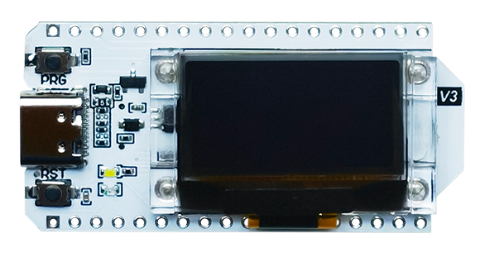
\includegraphics[width=0.25\linewidth]{figures/esp32heltec.png}
  \caption{Microcontrolador ESP32 con OLED integrado}
  \label{figure:esp32heltec}
\end{figure}

\section{C++}


El uso de C++ como tecnología de programación juega un papel fundamental. Este lenguaje de programación de alto nivel es ampliamente reconocido por su balance entre eficiencia y facilidad de uso, lo que lo convierte en una elección idónea para la programación de sistemas embebidos como el ESP32.

Las razones para utilizar C++ en este proyecto son las siguientes:

\begin{itemize}
   \item Eficiencia y control
   \item Programación orientada a objetos (OOP)
   \item Compatibilidad con librerías y jerramientas
   \item Extensa comunidad y recursos disponibles
\end{itemize}

A pesar de sus ventajas, programar en C++ también conlleva desafíos, especialmente en el contexto de sistemas embebidos. La gestión manual de la memoria y la complejidad inherente del lenguaje pueden aumentar el riesgo de errores. Por ello, es fundamental un entendimiento profundo de los conceptos de C++ y las mejores prácticas en su aplicación.


%%%%%%%%%%%%%%%%%%%%%%%%%%%%%%%%%%%%%%%%%%%%%%%%%%%%%%%%%%

\newpage{\pagestyle{empty}}
\thispagestyle{empty}

\chapter{\LARGE Desarrollo del proyecto}
\label{chapter:projectDevelopment}

En este capítulo se describe el desarrollo del código desarrollado, desde la primera versión del juego Snake hasta la versión final. Se explican los principales problemas encontrados y las soluciones propuestas para resolverlos. Además, se detallan las principales funciones y estructuras de datos utilizadas en el código.

\section{Version 1: Snake en C++ para ordenadores de escritorio}

La primera versión del juego Snake se desarrolló en C++ utilizando la librería estándar de C++ (STL). El objetivo de esta versión era crear un juego funcional que pudiera ser ejecutado en ordenadores de escritorio. El código se desarrolló en Visual Studio Code, que ofrece una interfaz gráfica intuitiva para escribir, compilar, depurar y ejecutar código C++.

\subsection{Estructura del código}

El código se divide en la siguiente estructura de carpetas:

\begin{itemize}
\item \textbf{src}: contiene los archivos de código fuente. Dónde se implementan las funciones.
\item \textbf{include}: contiene los archivos de cabecera. Dónde se declaran las funciones y variables.
\item \textbf{bin}: contiene los archivos ejecutables.
\end{itemize}


\subsection{Clases y estructuras de datos}

El código se divide en las siguientes clases y estructuras de datos:

\subsubsection{Clase \texttt{Board}}

La clase \texttt{Board} representa el tablero de juego en la implementación del juego Snake. Esta clase es fundamental para gestionar la lógica del juego, incluyendo el estado del tablero, la posición y movimiento de la serpiente, y la generación de alimentos.

Atributos y Métodos:

\begin{itemize}
    \item \textbf{Enumeración Square:} Define los posibles estados de cada cuadrado del tablero: vacío, comida, cuerpo de la serpiente y cabeza de la serpiente.
    \item \textbf{Constructores y Destructor:} La clase proporciona constructores para inicializar el tablero con dimensiones específicas y un destructor para la gestión adecuada de recursos.
    \item \textbf{Getters:} Métodos para obtener información sobre el tablero, como su ancho, alto y el estado de los cuadrados.
    \item \textbf{Métodos de Verificación:} Incluye funciones para verificar si una posición específica en el tablero corresponde a un borde, comida, cuerpo o cabeza de la serpiente.
    \item \textbf{turnGame y moveSnake:} Métodos para manejar el turno del juego y el movimiento de la serpiente, respectivamente.
    \item \textbf{Generación y Consumo de Comida:} Métodos para generar comida en el tablero y manejar su consumo por parte de la serpiente. La generación de comida se realiza de forma aleatoria y asegurando que no se genere en la posición actual de la serpiente.
    \item \textbf{gameOver:} Método para manejar el fin del juego.
    \item \textbf{Sobrecarga de Operadores:} Sobrecarga del operador de índice para acceder a los estados de los cuadrados del tablero y del operador de inserción para imprimir el tablero.
    \item \textbf{displayBoard:} Método para mostrar el tablero en un gestor de visualización.
\end{itemize}

Estructura Interna: 

\begin{itemize}
    \item \textbf{Atributos Privados:} Incluyen dimensiones del tablero, un puntero a un vector de vectores representando el estado de cada cuadrado, y un puntero a la instancia de la serpiente.
    \item \textbf{Métodos Privados:} Métodos para cambiar el estado de los cuadrados del tablero en respuesta a los movimientos de la serpiente.
\end{itemize}

Funcionalidad:

La clase \texttt{Board} actúa como el núcleo lógico del juego, manteniendo el estado del tablero y respondiendo a las interacciones del jugador y a los cambios en el juego. Su diseño modular y su conjunto de métodos bien definidos facilitan la gestión del estado del juego y la interacción con otros componentes, como la serpiente y el sistema de visualización.


\subsubsection{Clase \texttt{Snake}}

La clase \texttt{Snake} es responsable de representar y gestionar la serpiente en el juego. Esta clase controla el movimiento, el crecimiento y las interacciones de la serpiente con otros elementos del juego como la comida y los límites del tablero.

Atributos y Métodos:

\begin{itemize}
    \item \textbf{Constructores y Destructor:} La clase \texttt{Snake} proporciona constructores para inicializar la serpiente con una posición de inicio y un destructor para manejar adecuadamente la liberación de recursos.
    \item \textbf{Getters:} Incluye un método para obtener el tamaño del cuerpo de la serpiente.
    \item \textbf{Métodos de Verificación:} Métodos para verificar si una posición dada corresponde a la cabeza o el cuerpo de la serpiente.
    \item \textbf{Interacciones de Juego:} Métodos para comprobar la presencia de comida y detectar colisiones, fundamentales para la lógica del juego.
    \item \textbf{Movimiento:} Un método para mover la serpiente en una dirección dada.
\end{itemize}

Estructura Interna:

\begin{itemize}
    \item \textbf{Atributos Privados:} Incluyen un puntero al tablero de juego, el tamaño del cuerpo de la serpiente, un vector de \texttt{DirectedPosition} que representa el cuerpo, y la posición dirigida de la cabeza.
    \item \textbf{Métodos Privados:} Funciones para manejar el crecimiento de la serpiente, cambiar su dirección, comprobar la dirección opuesta, y mover el cuerpo y la cabeza de la serpiente.
\end{itemize}

Funcionalidad:

La clase \texttt{Snake} es esencial en la mecánica del juego, gestionando el estado y el comportamiento de la serpiente. Controla el movimiento, el crecimiento al consumir comida, y la detección de colisiones, que son aspectos críticos del juego. Su diseño permite una interacción efectiva con la clase \texttt{Board} y otros componentes del juego, asegurando una experiencia de juego coherente y fluida.

\subsubsection{Clases Auxiliares}

Las clases \texttt{DirectedPosition} y \texttt{Square} son componentes auxiliares en la implementación del juego Snake, proporcionando funcionalidades clave para la gestión de posiciones y el manejo las casillas, respectivamente.

Clase DirectedPosition:

La clase \texttt{DirectedPosition} encapsula la posición y dirección de un objeto en el juego, como podría ser un segmento de la serpiente o un ítem de comida.

La clase \texttt{Square} representa un cuadrado en el tablero de juego. Esta clase es fundamental para la gestión del estado del tablero, incluyendo la generación de comida y la detección de colisiones.


Funcionalidad y Aplicación:

Estas clases auxiliares desempeñan roles cruciales en la lógica del juego. \texttt{DirectedPosition} facilita el seguimiento y control de posiciones y direcciones de manera eficiente, mientras que \texttt{Vector} proporciona una forma sencilla de manejar en todo momento el estado de una casilla, haciendo que una casilla pueda ser sustituida por otro tipo de casillas en un futuro. Su uso mejora la claridad y modularidad del código, contribuyendo a una implementación más organizada y mantenible del juego Snake.

Se puede visualizar el resultado de la primera versión del juego Snake en la Figura \ref{figure:snakeV1}.

\begin{figure}[!htb]
   \centering
    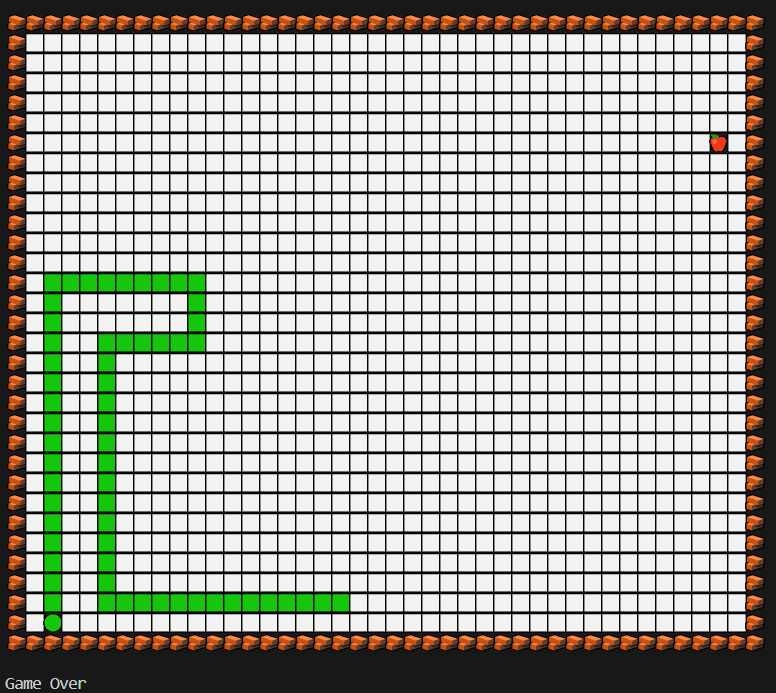
\includegraphics[width=0.6\linewidth]{figures/snakeV1.png}
   \caption{Versión del juego Snake para ordenadores de escritorio}
   \label{figure:snakeV1}
\end{figure}

\section{Version 2: Snake en ESP32 con C++ y Arduino IDE}

Esta versión del juego Snake, implementada en el microcontrolador ESP32 utilizando C++ y Arduino IDE, representa un esfuerzo inicial para explorar la flexibilidad y eficiencia de códigos modulares en plataformas de sistemas embebidos. Esta versión se centra en la legibilidad y la facilidad de modificación del código, aprovechando las capacidades de C++ y la estructura modular proporcionada por las clases dichas anteriormente.

Se ha añadido lo siguiente:

\begin{itemize}
  \item \textbf{Directorio libraries:} Creada automaticamente por Arduino IDE, contiene las librerías utilizadas en el proyecto.
  \item \textbf{Fichero minigames.ino:} Contiene el código principal del juego, incluyendo la configuración de la pantalla OLED y la inicialización de los objetos.
\end{itemize}

\subsection{Rendimiento y Desafíos Encontrados}

Aunque esta versión cumple con los objetivos básicos del juego, se identificaron varios desafíos y limitaciones durante su desarrollo y prueba:

\begin{itemize}
    \item \textbf{Uso de Memoria:} Aunque en principio no parece que la memoria sea un problema, cuando se intentaba ejecutar el juego en el ESP32, más especificamente, se intentaba acceder a una casilla por primera vez, el programa se reiniciaba. Se probó con diferentes tamaños de tablero, pero el problema persistía. Esto sugiere que la matriz no era el problema, sino que a lo mejor lo fue la pila de llamadas, ya que para dibujar cada casilla en la OLED se necesitaba pasar por varios objetos en cadena.
    \item \textbf{Escalabilidad:} A pesar de la modularidad del código, la escalabilidad del juego para incorporar características adicionales es totalmente limitada debido a la gestión de memoria y rendimiento.
\end{itemize}



\subsection{Conclusiones y Lecciones Aprendidas}

Esta primera versión del juego Snake en ESP32 ha sido instrumental para comprender las capacidades y limitaciones del ESP32 en el contexto de programación modular. Las lecciones aprendidas de esta implementación proporcionan una base sólida para futuras mejoras y optimizaciones, destacando la importancia de una gestión de memoria más eficiente y la necesidad de estrategias de optimización del rendimiento en sistemas embebidos.


\section{Version 3: Snake en ESP32 simplificado}

La segunda versión del juego Snake presenta una estructura simplificada, manteniendo la separación de la lógica del juego en distintos directorios como \texttt{src} e \texttt{include}, pero con una organización y un enfoque más eficientes.

\textbf{Simplificación de la Estructura:} Se ha eliminado gran parte de la escalabilidad y la modularidad del código para centrarse en la eficiencia y la estabilidad, lo que ha permitido una reducción significativa del uso de memoria. Basicamente se han eliminado todas las clases, y se ha pasado a utilizar dos ficheros .cpp y .h, uno para el funcionamiento del juego y otro para la serpiente.

\subsection{Estructura del Código}

La nueva estructura del código se muestra a continuación:

\begin{itemize}
    \item \textbf{Archivo Principal snake\_game.ino:} Este archivo sirve como punto de entrada del juego. Contiene la configuración inicial del microcontrolador ESP32 y la lógica principal para la ejecución del juego.
    
    \item \textbf{Directorio include/:} Contiene los archivos de cabecera, que definen las clases y las funciones utilizadas en el juego.
    \begin{itemize}
        \item \texttt{game.h:} Define las funciones que tienen que ver con el juego.
        \item \texttt{images.h:} Contiene definiciones de los bitmaps que representan logos y simbolos dibujados en bits.
        \item \texttt{snake.h:} Define las funciones que tienen que ver con la serpiente. Gestiona el comportamiento y el estado de la serpiente dentro del juego.
    \end{itemize}
    
    \item \textbf{Directorio src/:} Alberga los archivos de código fuente, donde se implementan las definiciones proporcionadas en los archivos de cabecera.
    \begin{itemize}
        \item \texttt{game.cpp:} Implementa la lógica de la clase Game, incluyendo el ciclo principal del juego y la gestión de eventos.
        \item \texttt{snake.cpp:} Contiene la implementación de la clase Snake, incluyendo la lógica de movimiento y crecimiento de la serpiente.
    \end{itemize}
    
    \item \textbf{Directorio libraries/:} Este directorio se utiliza para almacenar las bibliotecas de terceros o personalizadas que se utilizan en el proyecto, lo que puede incluir herramientas para la gestión de la pantalla OLED, la conectividad o el manejo de gráficos.
\end{itemize}

La organización de los archivos en esta estructura modular facilita el mantenimiento y la escalabilidad del código. Permite una separación clara entre la lógica del juego, la definición de las entidades y la implementación de funcionalidades específicas, lo que resulta en un código más limpio y fácil de entender.


\begin{itemize}
    \item \textbf{Directorio src:} Contiene los ficheros .cpp del juego. Dónde se implementan las funciones.
    \item \textbf{Directorio include:} Contiene los ficheros .h del juego. Dónde se declaran las funciones y variables.
    \item \textbf{Fichero minigame.ino:} Contiene el código principal del juego, incluyendo la configuración de la pantalla OLED y la inicialización de los objetos.

\subsection{Rendimiento y Eficiencia}

La revisión de la estructura del código ha tenido un impacto positivo en el rendimiento general del juego:

\begin{itemize}
    \item \textbf{Reducción del Uso de Memoria:} La nueva versión utiliza la memoria de manera más eficiente, lo que es crucial para el funcionamiento estable en el microcontrolador ESP32.
    \item \textbf{Estabilidad Mejorada:} Se observó una mejora significativa en la estabilidad durante las pruebas de juego extendidas, evidenciando la eficacia de las optimizaciones realizadas.
    \item \textbf{Escalabilidad:} La estructura simplificada y modular facilita la incorporación de nuevas características y la adaptación a diferentes plataformas o configuraciones de hardware.
    \item \textbf{Capacidad de testeo:} La modularidad del código permite una mayor facilidad de testeo, al disponer diferentes directorios y estructura dividida en declaración/implementación dada por el .h .cpp.
\end{itemize}

En la siguiente figura se muestra el juego en funcionamiento en la ESP32, con una pantalla OLED de 128x64 píxeles \ref{figure:snakeV2} y \ref{figure:snakeV2-1}.

\begin{figure}[!htb]
  \centering
   \includgraphics[width=0.6\linewidth]{figures/snakeV2.jpg}
  \caption{Versión del juego Snake para ESP32}
  \label{figure:snakeV2}
\end{figure}

\begin{figure}[!htb]
  \centering
   \includgraphics[width=0.6\linewidth]{figures/snakeV2.jpg}
  \caption{Versión del juego Snake para ESP32}
  \label{figure:snakeV2-1}
\end{figure}

El resultado de los bitmaps se puede ver en la figura \ref{figure:death} y \ref{figure:start}.

\begin{figure}[!htb]
  \centering
   \includgraphics[width=0.6\linewidth]{figures/death.jpg}
  \caption{Bitmap de la muerte cuando se pierde en el juego}
  \label{figure:death}
\end{figure}

\begin{figure}[!htb]
  \centering
   \includgraphics[width=0.6\linewidth]{figures/start.jpg}
  \caption{Bitmap para comenzar el juego}
  \label{figure:start}
\end{figure}

\subsection{Conclusiones y Perspectivas Futuras}

La segunda versión del juego Snake demuestra que las mejoras en la estructura del código y la integración eficiente de bibliotecas pueden tener un impacto sustancial en el rendimiento y la escalabilidad. Esta versión sirve como un ejemplo valioso de cómo la optimización y la simplificación pueden mejorar significativamente la viabilidad de proyectos de sistemas embebidos en plataformas como el ESP32.

Las lecciones aprendidas y las metodologías aplicadas en esta versión ofrecen una perspectiva valiosa para futuros proyectos que buscan equilibrar la eficiencia de recursos con la funcionalidad y la estabilidad en sistemas embebidos.


%%%%%%%%%%%%%%%%%%%%%%%%%%%%%%%%%%%%%%%%%%%%%%%%%%%%%%%%%
\newpage{\pagestyle{empty}}
\thispagestyle{empty}

\chapter{\LARGE Analisis de la experimentación y resultados obtenidos}
\label{chapter:analysisTestAndResults}

\section{Reinicios del ESP32}

Durante el desarrollo del proyecto, han habido una serie de reinicios que han dificultado la depuración del código. Muchas veces dado al desconocimiento del propio microcontrolador y otros por la primera versión del juego realizada.

\section{Manejo de la pantalla OLED}

La pantalla OLED es una de las partes más importantes del proyecto, ya que es la que muestra el juego. Hubieron varios problemas con la pantalla OLED, ya que no se sabía cómo manejarla. Se tuvo que investigar cómo funcionaba y cómo se podía utilizar.




%%%%%%%%%%%%%%%%%%%%%%%%%%%%%%%%%%%%%%%%%%%%%%%%%%%%%%%%%
\newpage{\pagestyle{empty}}
\thispagestyle{empty}

\chapter{\LARGE Conclusiones y líneas futuras}
\label{chapter:Resultados}

\section{Conclusiones}

En este apartado se presentan las conclusiones m\'as importantes de este trabajo. 

En primer lugar, se ha de destacar que se han cumplido todos los objetivos aunque no todo haya salido como se esperaba.

Este proyecto ha demostrado la viabilidad de implementar un juego clásico como Snake en un microcontrolador ESP32, destacando la importancia de la modularidad y eficiencia en la programación de sistemas embebidos.

\subsection{Lineas de Trabajo Futuras}

Este trabajo abre varias vías para investigaciones futuras y desarrollos en el campo de la programación de sistemas embebidos.

\begin{itemize}
    \item \textbf{Exploración de Otras Plataformas y Tecnologías:} Sería interesante replicar este estudio en diferentes plataformas de microcontroladores para comparar rendimientos y capacidades.
    \item \textbf{Integración de Funcionalidades Avanzadas:} Existe un potencial para expandir el juego con características adicionales, como conectividad en red o inteligencia artificial, para explorar más a fondo las capacidades del ESP32.
\end{itemize}

\subsection{Reflexiones Finales}

El desarrollo del juego Snake en el ESP32 ha proporcionado una valiosa experiencia en la programación de sistemas embebidos, destacando tanto los desafíos como las oportunidades en este campo. Este proyecto no solo contribuye al conocimiento académico en el área de sistemas embebidos, sino que también ofrece perspectivas prácticas aplicables a una variedad de aplicaciones en el mundo real.

%%%%%%%%%%%%%%%%%%%%%%%%%%%%%%%%%%%%%%%%%%%%%%%%%%%%%%%%%
\newpage{\pagestyle{empty}}
\thispagestyle{empty}

\chapter{\LARGE Conclusions and future lines}
\label{chapter:Conclusiones}

\section{Conclusions}

This section presents the most important conclusions of this work.

Firstly, it should be highlighted that all objectives have been met, although not everything went as expected.

This project has demonstrated the feasibility of implementing a classic game like Snake on an ESP32 microcontroller, highlighting the importance of modularity and efficiency in programming embedded systems.

\subsection{Future Lines of Work}

This work opens several avenues for future research and developments in the field of embedded systems programming.

\begin{itemize}
    \item \textbf{Exploration of Other Platforms and Technologies:} It would be interesting to replicate this study on different microcontroller platforms to compare performance and capabilities.
    \item \textbf{Integration of Advanced Features:} There is potential to expand the game with additional features, such as network connectivity or artificial intelligence, to further explore the capabilities of the ESP32.
\end{itemize}

\subsection{Final Reflections}

The development of the Snake game on the ESP32 has provided valuable experience in the programming of embedded systems, highlighting both the challenges and opportunities in this field. This project not only contributes to academic knowledge in the area of embedded systems but also offers practical perspectives applicable to a variety of real-world applications.


%%%%%%%%%%%%%%%%%%%%%%%%%%%%%%%%%%%%%%%%%%%%%%%%%%%%%%%%%
\newpage{\pagestyle{empty}}
\thispagestyle{empty}

\chapter{\LARGE Bibliografía}
\label{chapter:Bibliografía}

%
%
\begingroup
\renewcommand{\section}[2]{}
\renewcommand{\chapter}[2]{}
\bibliographystyle{apalike}
\bibliography{memtfg.bib}
\endgroup

%%%%%%%%%%%%%%%%%%%%%%%%%%%%%%%%%%%%%%%%%%%%%%%%%%%%%%%%%%

%\begin{thebibliography}{X}
% Aquí figurará la bibliografía
%\end{thebibliography}

%%%%%%%%%%%%%%%%%%%%%%%%%%%%%%%%%%%%%%%%%%%%%%%%%%%%%%%%%

\newpage{\pagestyle{empty}\cleardoublepage}
\thispagestyle{empty}

\begin{appendix}


\chapter{\LARGE Códigos relevantes del proyecto}
\label{appendix:1}
Github: \url{https://github.com/anabeldilab/ESP32_snakeGame}


\end{appendix}

\end{document}

